\documentclass[12pt,twoside]{article}
\usepackage{tikz}
\usepackage[siunitx]{circuitikz}
\usepackage{siunitx}
\usepackage{systeme}
\usepackage{graphicx}
\usepackage{listings}
\usepackage{float}

\begin{document}

\title{\textbf{Tema 01\\
{\small - la disciplina Bazele Electrotehnicii - }}}


\author{{\em Apostolescu Mihnea}
\\ mihnea.apostolescu@stud.acs.upb.ro   \\
312AC Anul I\\
Facultatea de Automatică și Calculatoare , UPB}

\date{\today}


\maketitle

\newpage
\tableofcontents

\newpage

\section{Generarea unui circuit}
\paragraph{}


Graful de intensități $\mathcal{G}_i$: 
\begin{center}
\begin{circuitikz}
\draw (4,4) to[short, i^<=5A] (8,4);
\draw (4,0) to[short, i_<=7A] (4,4);
\draw (0,0) to (4,0);
\draw (0,0) to[short, i_>=2A] (0,4);
\draw (0,4) to (4,4);
\draw (8,4) to[short, i_<=3A] (8,0);
\draw (8,0) to[short, i_<=5A] (4,0);
\draw (8,0) to (12,0);
\draw (12,0) to[short, i_>=2A] (12,4);
\draw (12,4) to (8,4);
\end{circuitikz}
\end{center}

Graful de intensități $\mathcal{G}_u$: 
\begin{center}
\begin{circuitikz}
\draw (4,4) to[short, i^>=5V] (8,4);
\draw (4,0) to[short, i^<=25V] (4,4);
\draw (0,0) to (4,0);
\draw (0,0) to[short, i_<=25V] (0,4);
\draw (0,4) to (4,4);
\draw (8,4) to[short, i^<=15V] (8,0);
\draw (8,0) to[short, i^>=35V] (4,0);
\draw (8,0) to (12,0);
\draw (12,0) to[short, i^>=15V] (12,4);
\draw (12,4) to (8,4);
\end{circuitikz}
\end{center}

\begin{center}
\begin{circuitikz}[american]
\draw[red] (4, 4) to[V<=5V , color=red] (8,4);
\draw[red] (4, 2) to[R, l_=$R_2$,a^=5<\ohm> , color=red]	(4,4);
\draw[red] (4, 0) to[V<=10V , color=red] (4, 2);
\draw (0, 0) to (4,0)
node[label={[font=\footnotesize]below:$(4)$}] {};
\draw (0, 0) to[I, i_>=$2$A] (0,2);
\draw (0, 2) to[R, l_=$R_1$,a^=6<\ohm>] (0,4);
\draw (0, 4) to (4,4)
node[label={[font=\footnotesize]above:$(1)$}] {};
\draw[red] (8, 4) to[R, l_=$R_5$,a^=5<\ohm> , color=red] (8,0)
node[label={[font=\footnotesize , color = black]below:$(3)$}] {};
\draw (8, 0) to[R, l_=$R_3$,a^=10<\ohm>] (6,0);
\draw (4, 0) to[I, i_>=$5$A] (6,0);
\draw (8, 0) to (12, 0);
\draw (12, 0) to[I, i_>=$2$A] (12,2);
\draw (12, 2) to[R, l_=$R_4$,a^=8<\ohm>] (12,4);
\draw (12, 4) to (8,4)
node[label={[font=\footnotesize]above:$(2)$}] {};
\end{circuitikz}
\end{center}

\section{Metode sistematice eficiente}
\paragraph{}

\begin{center}
\begin{tabular}{|m{10cm}|m{5cm}|}
\hline
Metodă & Număr de ecuații\\
\hline\hline
Kirchhoff clasic & $2L = 12$\\
\hline
Kirchhoff în curenți & $L - N + 1 = 3$\\
\hline
Kirchhoff în tensiuni & $N - 1 = 3$\\
\hline
Curenți în coarde  (curenți de bucle/curenți ciclici) & $L - N + 1 - n_{SIC} = 3$\\
\hline
Tensiuni în ramuri (potențiale ale nodurilor dacă SIT formează un subgraf conex)& $N - 1 - n_{SIT} = 2$\\
\hline

\end{tabular}
\end{center}

\begin{flushleft}
Metoda tensiunilor în ramuri este cea mai eficientă.
\\ Vom folosi această metodă pentru a rezolva circuitul de mai sus.
\end{flushleft}
Arborele normal are $N - 1 = 3$ ramuri.
\\Ramurile rosii din desen fac parte din arbore.


Avem $N - 1 - n_{SIT} = 2$ secțiuni :

\vspace{10px}
\{1\} = \{$coarda (4) \rightarrow (1),\quad coarda (4) \rightarrow (3) ,\quad ramura (1) \rightarrow (4)$\}

\{2\} = \{$coarda (4) \rightarrow (3) ,\quad ramura (3) \rightarrow (2) , \quad coarda (3) \rightarrow (2)$\}

\vspace{10px}
\begin{flushleft}
Alegem sensuri de referință arbitrare pentru curenți și scriem \textit{Teoreme Kirchhoff I} pentru secțiunile alese.
\end{flushleft} 

Vom obține urmatorul sistem de ecuații :

\begin{equation}
\systeme*{
\{1\}: \frac{U_{14} + 10}{5} - 2 - 5 = 0,
\{2\}: 5 - \frac{U_{32}}{10} - 2 = 0
}
\end{equation}

\vspace{10px}
Rezolvând acest sistem de ecuații vom obține $U_{14}=25V$ și $U_{32}=15V$, valori identice cu cele din graful de tensiuni prezentat la început (cu valorile preluate din LTSpice).  

\newpage
\section{Generatorul echivalent de tensiune/curent}
\paragraph{}

\subsection{Dependența curentului, tensiunii și puterii prin rezistor
în funcție de valoarea rezistenței}
\paragraph{}

\subsection{Punctul static de funcționare (SRT + Rezistor)}
\paragraph{}

\subsection{Punctul static de funcționare (SRT + Diodă semiconductoare)}
\paragraph{}

\section{Surse comandate}
\paragraph{}

\subsection{Circuit cu SUCU}
\paragraph{}

\begin{center}
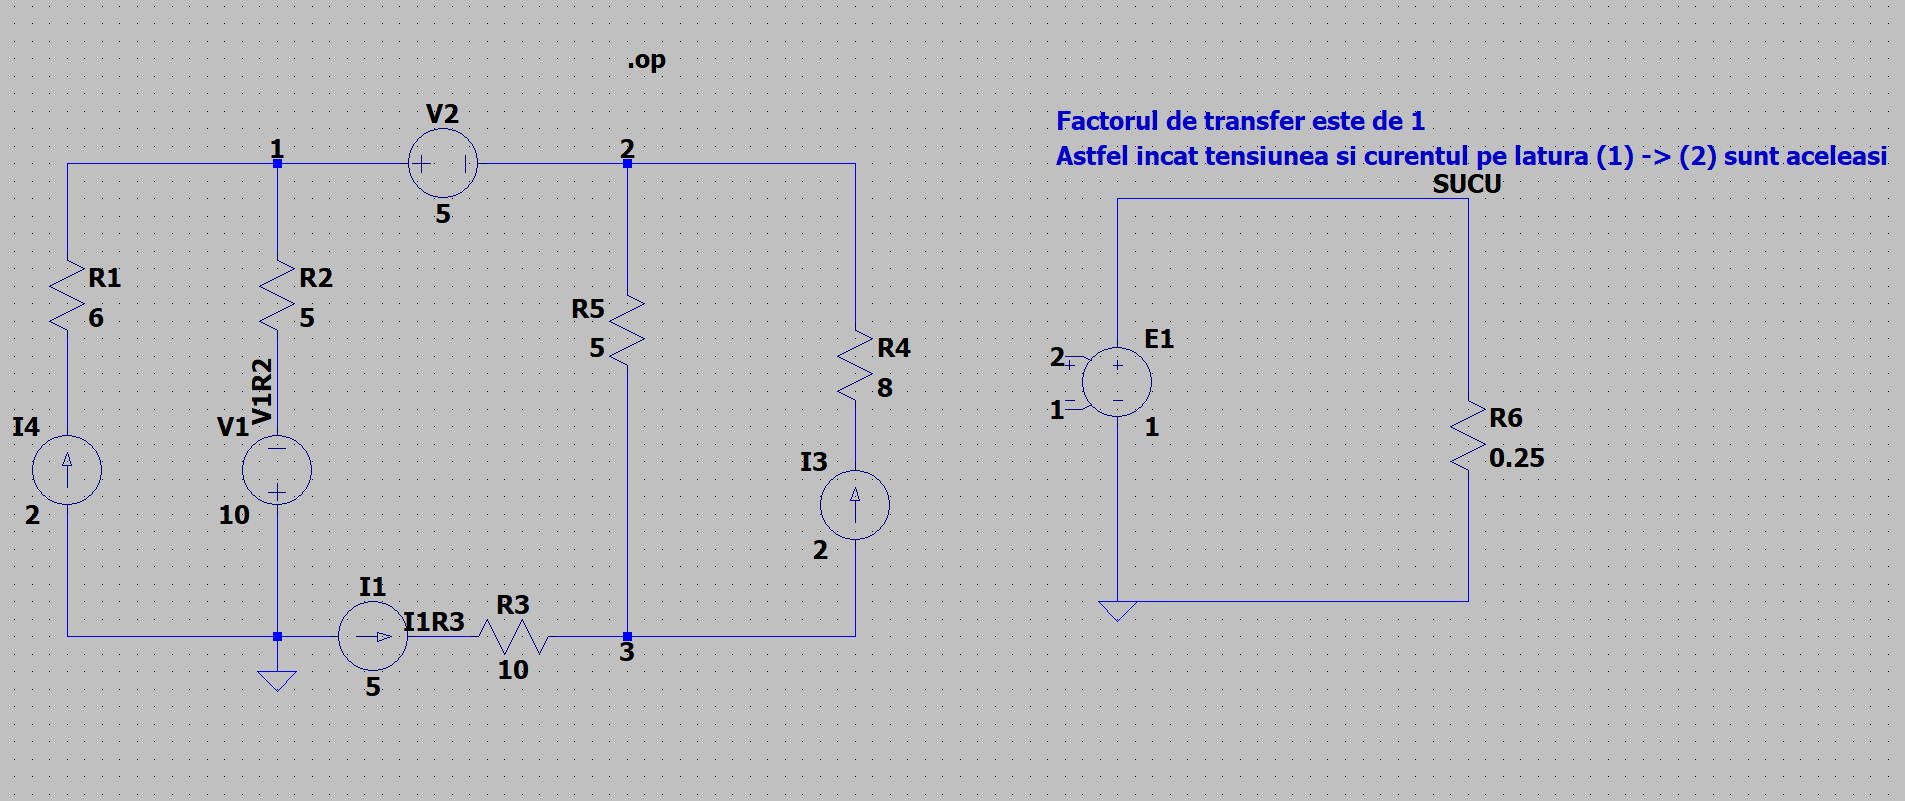
\includegraphics[scale=0.25]{SUCU_tema_elth.png}
\end{center}


\subsection{Simulare SPICE}
\paragraph{}
Mai jos urmează simularea de rulare a circuitului in LTSpice:
\begin{center}
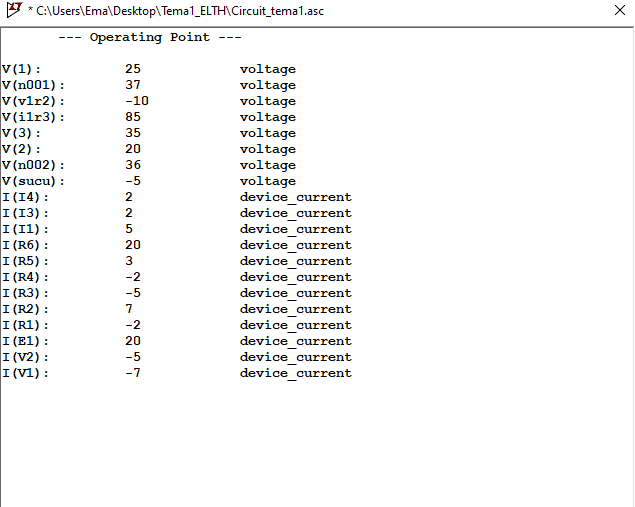
\includegraphics[scale=0.5]{simulation_spice.png}
\end{center}

\section{Rezolvarea circuitelor de curent alternativ}
\paragraph{}

Formăm circuitul în complex dupa cerințele date:

\begin{center}
\begin{circuitikz}[american]
\draw[red] (4, 4) to[V<=5V , color=red] (8,4);
\draw[red] (4, 2) to[R, l_=$R_2$,a^=5<\ohm> , color=red]	(4,4);
\draw[red] (4, 0) to[V<=10V , color=red] (4, 2);
\draw (0, 0) to (4,0)
node[label={[font=\footnotesize]below:$(4)$}] {};
\draw (0, 0) to[I, i_>=$2$A] (0,2);
\draw (0, 2) to[R, l_=$R_1$,a^=6<\ohm>] (0,4);
\draw (0, 4) to (4,4)
node[label={[font=\footnotesize]above:$(1)$}] {};
\draw[red] (8, 4) to[R, l_=$R_5$,a^=5<\ohm> , color=red] (8,0)
node[label={[font=\footnotesize , color = black]below:$(3)$}] {};
\draw (8, 0) to[R, l_=$R_3$,a^=10<\ohm>] (6,0);
\draw (4, 0) to[I, i_>=$5$A] (6,0);
\draw (8, 0) to (12, 0);
\draw (12, 0) to[I, i_>=$2$A] (12,2);
\draw (12, 2) to[R, l_=$R_4$,a^=8<\ohm>] (12,4);
\draw (12, 4) to (8,4)
node[label={[font=\footnotesize]above:$(2)$}] {};
\end{circuitikz}
\end{center}

\end{document}
